\documentclass[11pt,]{article}
\usepackage[left=1in,top=1in,right=1in,bottom=1in]{geometry}
\newcommand*{\authorfont}{\fontfamily{phv}\selectfont}
\usepackage[]{mathpazo}


  \usepackage[T1]{fontenc}
  \usepackage[utf8]{inputenc}



\usepackage{abstract}
\renewcommand{\abstractname}{}    % clear the title
\renewcommand{\absnamepos}{empty} % originally center

\renewenvironment{abstract}
 {{%
    \setlength{\leftmargin}{0mm}
    \setlength{\rightmargin}{\leftmargin}%
  }%
  \relax}
 {\endlist}

\makeatletter
\def\@maketitle{%
  \newpage
%  \null
%  \vskip 2em%
%  \begin{center}%
  \let \footnote \thanks
    {\fontsize{18}{20}\selectfont\raggedright  \setlength{\parindent}{0pt} \@title \par}%
}
%\fi
\makeatother




\setcounter{secnumdepth}{3}

\usepackage{longtable,booktabs}

\usepackage{graphicx,grffile}
\makeatletter
\def\maxwidth{\ifdim\Gin@nat@width>\linewidth\linewidth\else\Gin@nat@width\fi}
\def\maxheight{\ifdim\Gin@nat@height>\textheight\textheight\else\Gin@nat@height\fi}
\makeatother
% Scale images if necessary, so that they will not overflow the page
% margins by default, and it is still possible to overwrite the defaults
% using explicit options in \includegraphics[width, height, ...]{}
\setkeys{Gin}{width=\maxwidth,height=\maxheight,keepaspectratio}

\title{Asociacion y composicion floristica de la familia Sapotaceae en la
parcela permanente de 50h, Isla Barro Colorado  }



\author{\Large Merali Rosario\vspace{0.05in} \newline\normalsize\emph{Afiliación, normalmente algo tal que ``Estudiante, Universidad Autónoma
de Santo Domingo (UASD)''}  }


\date{}

\usepackage{titlesec}

\titleformat*{\section}{\normalsize\bfseries}
\titleformat*{\subsection}{\normalsize\itshape}
\titleformat*{\subsubsection}{\normalsize\itshape}
\titleformat*{\paragraph}{\normalsize\itshape}
\titleformat*{\subparagraph}{\normalsize\itshape}

\titlespacing{\section}
{0pt}{36pt}{0pt}
\titlespacing{\subsection}
{0pt}{36pt}{0pt}
\titlespacing{\subsubsection}
{0pt}{36pt}{0pt}





\newtheorem{hypothesis}{Hypothesis}
\usepackage{setspace}

\makeatletter
\@ifpackageloaded{hyperref}{}{%
\ifxetex
  \PassOptionsToPackage{hyphens}{url}\usepackage[setpagesize=false, % page size defined by xetex
              unicode=false, % unicode breaks when used with xetex
              xetex]{hyperref}
\else
  \PassOptionsToPackage{hyphens}{url}\usepackage[unicode=true]{hyperref}
\fi
}

\@ifpackageloaded{color}{
    \PassOptionsToPackage{usenames,dvipsnames}{color}
}{%
    \usepackage[usenames,dvipsnames]{color}
}
\makeatother
\hypersetup{breaklinks=true,
            bookmarks=true,
            pdfauthor={Merali Rosario (Afiliación, normalmente algo tal que ``Estudiante, Universidad Autónoma
de Santo Domingo (UASD)'')},
             pdfkeywords = {palabra clave 1, palabra clave 2},  
            pdftitle={Asociacion y composicion floristica de la familia Sapotaceae en la
parcela permanente de 50h, Isla Barro Colorado},
            colorlinks=true,
            citecolor=blue,
            urlcolor=blue,
            linkcolor=magenta,
            pdfborder={0 0 0}}
\urlstyle{same}  % don't use monospace font for urls

% set default figure placement to htbp
\makeatletter
\def\fps@figure{htbp}
\makeatother

\usepackage{pdflscape} \newcommand{\blandscape}{\begin{landscape}}
\newcommand{\elandscape}{\end{landscape}} \usepackage{float}
\floatplacement{figure}{H}
\newcommand{\beginsupplement}{ \setcounter{table}{0} \renewcommand{\thetable}{S\arabic{table}} \setcounter{figure}{0} \renewcommand{\thefigure}{S\arabic{figure}} }


% add tightlist ----------
\providecommand{\tightlist}{%
\setlength{\itemsep}{0pt}\setlength{\parskip}{0pt}}

\begin{document}
	
% \pagenumbering{arabic}% resets `page` counter to 1 
%
% \maketitle

{% \usefont{T1}{pnc}{m}{n}
\setlength{\parindent}{0pt}
\thispagestyle{plain}
{\fontsize{18}{20}\selectfont\raggedright 
\maketitle  % title \par  

}

{
   \vskip 13.5pt\relax \normalsize\fontsize{11}{12} 
\textbf{\authorfont Merali Rosario} \hskip 15pt \emph{\small Afiliación, normalmente algo tal que ``Estudiante, Universidad Autónoma
de Santo Domingo (UASD)''}   

}

}








\begin{abstract}

    \hbox{\vrule height .2pt width 39.14pc}

    \vskip 8.5pt % \small 

\noindent Resumen del manuscrito


\vskip 8.5pt \noindent \emph{Keywords}: palabra clave 1, palabra clave 2 \par

    \hbox{\vrule height .2pt width 39.14pc}



\end{abstract}


\vskip 6.5pt


\noindent  \section{Introducción}\label{introducciuxf3n}

La diversidad y estructura de los bosques miden los recursos y la
abundancia en un área geográfica, por ejemplo, los bosques de la familia
Sapotaceae son importantes para proporcionar alimento a las especies de
vida silvestre (Martínez-Sovero et al., 2021). La familia Sapotaceae
está ampliamente distribuida en la zonas tropicales (Smedmark, 2007).
Produce madera de alta calidad, frutas tropicales y algunas especies
producen látex, siendo una familia de plantas de importancia ecológica y
económica (Martínez-Sovero, Iglesias-Osores, \& Villena-Velásquez,
2020).

La Isla Barro Colorado es una reserva natural ubicada en el lago Gatún
del Canal de Panamá. Debido a su capacidad de investigación, es una de
las regiones tropicales más conocidas en materia de biología y ecología
tropical (``Isla barro colorado y biología tropical,'' 1990). La isla
exhibe características importantes, tres de las cuales son la
estabilidad ambiental, su ubicación geográfica (en un área de
importancia internacional) y la capacidad para investigar grupos
específicos de organismos (Rodríguez-Flores \& Barrios, 2020). Sin
embargo, no se han hecho estudios completos de la familia Sapotaceae,
donde se estudie los diferentes analisis de ecologia numerica.

El objetivo de este trabajo es determinar la asociacion, composicion
floristica y distribucion de la familia Sapotaceae en la parcela
permanente de 50h de la isla Barro Colorado. Ademas, analizar la
organizacion de las especies en los cuadros de 1 hectárea e identificar
si existe algun patron con alguna variable ambiental, asi como tambien,
explicar si hay especies indicadoras o con preferencia por determinadas
condiciones ambientales. Por otra parte, evaluar si la familia
sapotaceae esta suficientemente representada segun los análisis de
estimación de riqueza, determinar cuales son las variables ambientales
que presentan asociacion con la diversidad alpha y mostrar cuales son
las especies que contribuyen a la diversidad beta. Por ultimo, pero no
menos importante, examinar la autocorrelación espacial de las especies.

\section{Metodología}\label{metodologuxeda}

\subsection{Area de Estudio}\label{area-de-estudio}

La isla de Barro Colorado es una colina de 1,500 hectáreas ubicada a 137
msnm en el lago Gatún. La parte superior de la isla es ancha y plana, y
se asienta sobre un lecho de roca de basalto, de la cual irradian
colinas empinadas y valles tallados en rocas sedimentarias que contienen
gran cantidad de restos volcánicos. El suelo es arcilloso y la
profundidad varía de 50 cm a un metro. El clima es típico de las areas
tropicales (Pérez et al., 2005; Windsor et al., n.d.). Su vegetación
está formada por bosques semideciduos de tierras bajas, y se han
registrado más de 1,300 especies de plantas vasculares (croata, 1978).

La parcela permanente de árboles de 50 hectáreas se estableció en 1980
en el bosque húmedo tropical. El sitio es un rectángulo de 1,000 m de
largo por 500 m de ancho, ubicado en la meseta central de la isla. Está
dividido en 1,250 cuadrantes de 20x20 m, en el cual se han contabilizado
todos los arboles con más de 10 mm de diámetro a la altura del pecho
cada cinco años desde 1985 (R. A. y H. Condit Richard y Chisholm, 2012;
R. y L. Condit Richard y P ~'e rez, 2017; Pérez et al., 2005).

\subsection{Maeriales y Metodos}\label{maeriales-y-metodos}

Los datos de cada uno de los cuadrantes de una hectárea que componen
BCI, fueron procesados en R (R Core Team, 2020), teniendo en cuenta la
matriz ambiental y la matriz de comunidad, los cuales contienen datos de
las variables ambientales, tales como condiciones edaficas, tipo de
habitat, topografia del lugar, clasificacion etaria del bosque, y datos
demográficos y geoferenciación espacial de todos los individuos
censados. Se adaptaron scripts reproducibles recuperados de Batlle
(2020), utilizando la colección de paquetes multifuncionales: vegan
(Oksanen et al., 2019), Tidyverse (Wickham, 2017), BiodiversityR (R.
Kindt \& Coe, 2005) y indicspecies (De Caceres \& Legendre, 2009).

Para conocer las características de los datos almacenados de la matriz
de comunidad y ambiental, se realizó un análisis exploratorio que
incluyó visualización de gráficos, tablas, mapas de los cuadrantes de
una hectárea y tablas de correlación lineal entre las dos variables de
la matriz, lo que permitió una vista común y ayudó a determinar
procedimientos más detallados a continuación.

\subsection{Medición de asociación
(ma)}\label{mediciuxf3n-de-asociaciuxf3n-ma}

Para realizar las pruebas de medicion de asociacion, se calculó la
distancia euclidiana entre los cuadrados considerados objetos. Para
ello, se requierió una transformación de la matriz de comunidad mediante
el método Hellinger, que incluye elevar al cuadrado la abundancia
relativa yij (cociente resultante de cada valor de abundancia entre la
suma de los sitios), como muestra la formula \ref{fig:formula}. Donde j
denota cada tipo o columna de la matriz, i es la fila o cuadrante e i+
representa la suma de filas de la matriz de la i-ésima fila (Legendre \&
Gallagher, 2001). Además, se evaluó la distancia euclidiana entre los
cuadrantes en términos de ocurrencia de especies. Se utilizó el índice
de disimilitud de Jaccard de la matriz normalizada para convertir el
valor de abundancia en un valor binario (Brocard, Gillet, \& Legendre,
2018). del mismo modo, se empleó la métrica de Jaccard para aplicar la
transposición de la matriz de la comunidad y convertir a datos Presencia
/ ausencia para medir el grado de asociación entre especies.

\begin{figure}
\centering
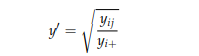
\includegraphics[width=1.00000\textwidth]{Formula2.png}
\caption{Formula. Transformación de la matriz de comunidad mediante el
método Hellinger \label{fig:formula}}
\end{figure}

Para poder comparar la relación entre especies en función de su
abundancia, se utilizó estandarización ji-cuadrado de la matriz de
comunidad transpuesta (Legendre \& Gallagher, 2001). Se examinó la
ocurrencia entre especies y su distribución en BCI por el coeficiente de
orrelación entre rangos de Spearman para medir el grado de correlación
entre las variables riqueza númerica de especies y la abundancia con las
variables ambientales geomorfológicas, y la composición química del
suelo(Brocard et al., 2018).

\subsection{Analisis de agrupamiento}\label{analisis-de-agrupamiento}

El método jerarquico aglomerativo de asociación entre pares de
cuadrantes (según la composición de especies) bajo el estándar de enlace
completo, y el método de Ward basado en la varianza mínima, se utilizan
como método preliminar para el análisis de agrupamiento, con el fin de
probar su efectividad en lograr un grupo consistente de importancia
ecológica (Brocard et al., 2018). Luego, estos generaron dendrogramas
que posteriormente son comparados con la matriz de distancia de cuerdas
(Legendre \& Gallagher, 2001). Usando correlación cofenética entre los
dos para determinar el número ideal de grupos. Además, se utilizó
remuestreo bootstrap y boostrap multiescalar para conocer la
probabilidad de éxito de la inferencia del número de grupos y la
identidad de sus componentes (Brocard et al., 2018). Las distribuciones
se basaban en una probabilidad de 91\% o más de acierto para el método
bootstrap y de un 95\% para boostrap multiescalar.

Dado que se localizaron patrones consistentes en la composicion y numero
de grupos entre los metodos examinados, los análisis de agruoamiento
posteriores se basan en los que se produce por enlace completo e incluye
dos grupos compuestos por 20 y 30 cuadrantes, respectivamente(ver figura
\ref{fig:Dendograma}).

\begin{figure}
\centering
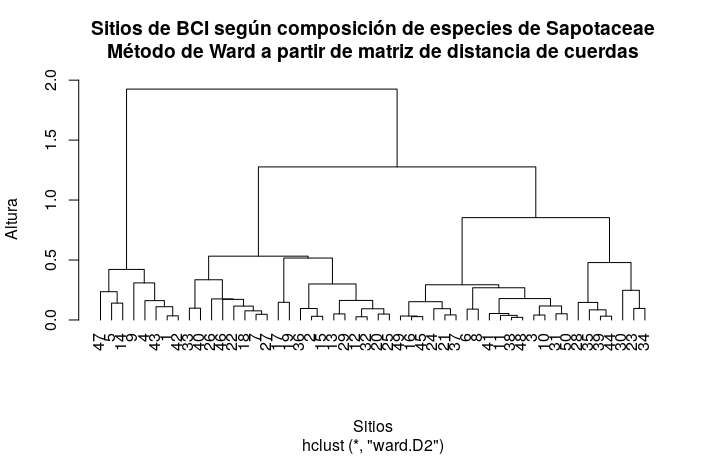
\includegraphics[width=1.00000\textwidth]{Dendograma.png}
\caption{Dendrogramas de los grupos producidos por Ward y Complete
\label{fig:Dendograma}}
\end{figure}

Para conocer las especies distintas o asociadas a cada grupo, se utilizo
el valor del indicador o índice IndVal (``Conjuntos de especies y
especies indicadoras,'' 1997), basado en permutaciones aleatorias de los
sitios según la presencia de especies y la abundancia de estos. De
manera similar, el grado de asociación de una especie con una
preferencia particular por el grupo de cuadrantes considerado grupo en
estudio, expresado como el coeficiente de correlación biserial puntual
(Brocard et al., 2018). Se adoptó un enfoque similar al anterior a lo
largo de las pruebas estadísticas de la hipótesis nula, basada en las
especies presentes en los cuadrantes pertenecientes a un determinado
grupo realizado al azar. Esta prueba se hizo reordenando aleatoriamente
los valores de abundancia y comparando sus distribuciones con las
obtenidas previamente (Cáceres \& Legendre, 2009).

\subsection{Análisis de diversidad
alpha}\label{anuxe1lisis-de-diversidad-alpha}

La diversidad alpha representa la diversidad de especies a lo largo de
todas las subunidades locales relevantes, y por definición abarca dos
variables importantes: (1) la riqueza de especies, y (2) la abundancia
relativa de especies (Carmona-Galindo \& Carmona, 2013). Para calcular
la diversidad alpha se utiliza el indice de Fisher (Fisher, Corbet, \&
Williams, 1943), el índice de Simpson (E. H. Simpson, 1949), y el índice
de Shannon-Wiener (Shannon, 1948). A fin de determinar la diversidad
alpha se utilizaron métodos como la Entropia de Shannon H1, que calcula
el grado de desorden en la muestra, el índice de concentración de
Simpson, que calcula la probabilidad de que dos individuos seleccionados
aleatoriamente puedan ser de la misma especie. Ademas, se empleó la
serie de números de diversidad de Hill, la fórmula de la entropía de
Rengi y el índice de equidad de Pielou.

Para determinar la rarefaccion se comparó los índices de diversidad
entre hábitats en base a un mismo número de individuos, donde el hábitat
con el mayor número de individuos se submuestreo sin remplazo
aleatoriamente y con múltiples ejecuciones para generar un índice
promedio que se pueda comparar con el índice de otro hábitat en base a
un mismo número de individuos. El resultado de esta técnica resulto con
una curva rarificada de valores del índice de diversidad que disminuye
conforme con el muestreo sin remplazo del número de
individuos(Carmona-Galindo \& Carmona, 2013)(ver figura
\ref{fig:Curva_rarefaccion} y
\ref{fig:acumulacion_especies_individuos}).

\subsection{Analisis de diversidad
beta}\label{analisis-de-diversidad-beta}

La diversidad beta, de acuerdo con (Whittaker, 1960), se define como el
diferencial entre la diversidad de un hábitat y la diversidad total de
un paisaje de hábitats. Teniendo en vuenta lo anterior, se utilizó el
metodo hellinger para determinar cuales son las especies que contribuyen
a la diversidad beta, es decir, las especies que no se encuentran
compartidas entre los cuadrantes.

\subsection{Análisis de ordenación simple (no restringida) y canónica
(restringida)}\label{anuxe1lisis-de-ordenaciuxf3n-simple-no-restringida-y-canuxf3nica-restringida}

Se aplicaron los análisis de componentes principales o PCA a los datos
de las variables ambientale para determianar la ordenacion no
restringida, donde se tomó en cuenta especificamente las variables del
suelo. y para determinar la ordenacion restringida se exploró de manera
explícita las relaciones entre una matriz de respuesta y una matriz
explicativa con los análisis de redundancia o RDA, lo cual combina la
regresión y el análisis de componentes principales (PCA), por ejemplo,
busca tendencias en la matriz de comunidad restringiéndolas a la matriz
ambiental.

\subsection{Ecología espacial}\label{ecologuxeda-espacial}

En ecología espacial se utilizó la matriz transformada de hellinger y la
matriz ambiental para crear un cuadro de vecindad y ver como se
autocorrelacionan los sitios. Se genera un correlograma para la variable
que queremos estudiar mediante la función `sp.correlogram' y para varias
variables como la abundancia de especies y las variables ambientales.
También, se utilizaron otros métodos como la prueba Mantel con matrices
de distancia para autocorrelación espacial con y sin tendencia, y el I
de Moran con una matriz de abundancia de especies transformada sin
tendencia, lo cual se aplica a variables ambientales para obtener los
datos de autocorrelación, distribución de especies y variables en los
sitios d muestreo.

\section{Resultados}\label{resultados}

Se registraron un total de 5 especies y 2 generos distribuidos en 2029
individuos en toda la parcela. La riqueza por cuadro fue de 4 especies y
la mediana de la abundancia por cuadro fue de 39 individuos. La especie
más abundante fue \emph{Pouteria reticulata}, con 1084 individuos, y la
menos abundante fue \emph{Pouteria fossicola} con 3 individuos. La tabla
\ref{tab:abun_sp} y la figura \ref{fig:abun_sp_q} resume estos
resultados. La distribucion de la riqueza númerica de especies de la
familia Sapotaceae sigue un patrón homogeneo, lo cual los agregados de
riqueza maxima estan distribuidos en casi todo el area (ver Figura
\ref{fig:mapa_cuadros_riq_mi_familia}).

\begin{longtable}[]{@{}lr@{}}
\caption{\label{tab:abun_sp}Abundancia por especie de la familia
Sapotaceae}\tabularnewline
\toprule
Latin & n\tabularnewline
\midrule
\endfirsthead
\toprule
Latin & n\tabularnewline
\midrule
\endhead
Pouteria reticulata & 1084\tabularnewline
Chrysophyllum argenteum & 711\tabularnewline
Chrysophyllum cainito & 171\tabularnewline
Pouteria stipitata & 60\tabularnewline
Pouteria fossicola & 3\tabularnewline
\bottomrule
\end{longtable}

\begin{figure}
\centering
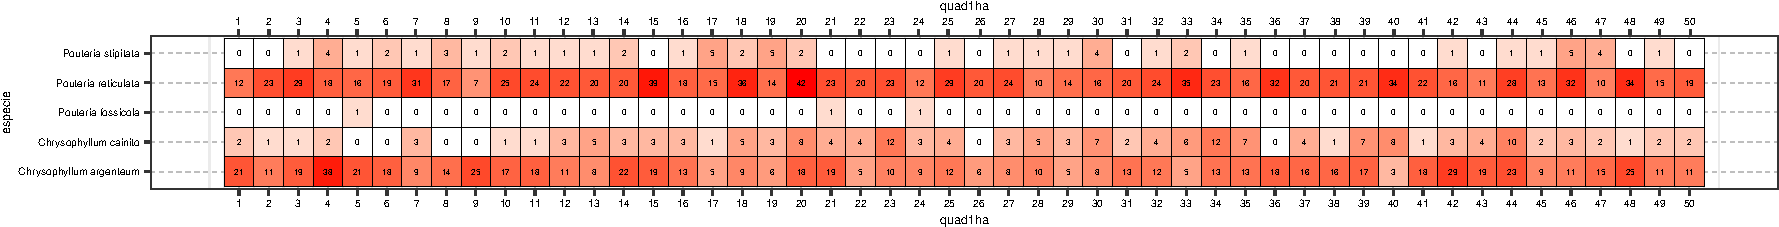
\includegraphics{manuscrito_files/figure-latex/unnamed-chunk-3-1.pdf}
\caption{\label{fig:abun_sp_q}Abundancia por especie por quadrat}
\end{figure}

\begin{figure}
\centering
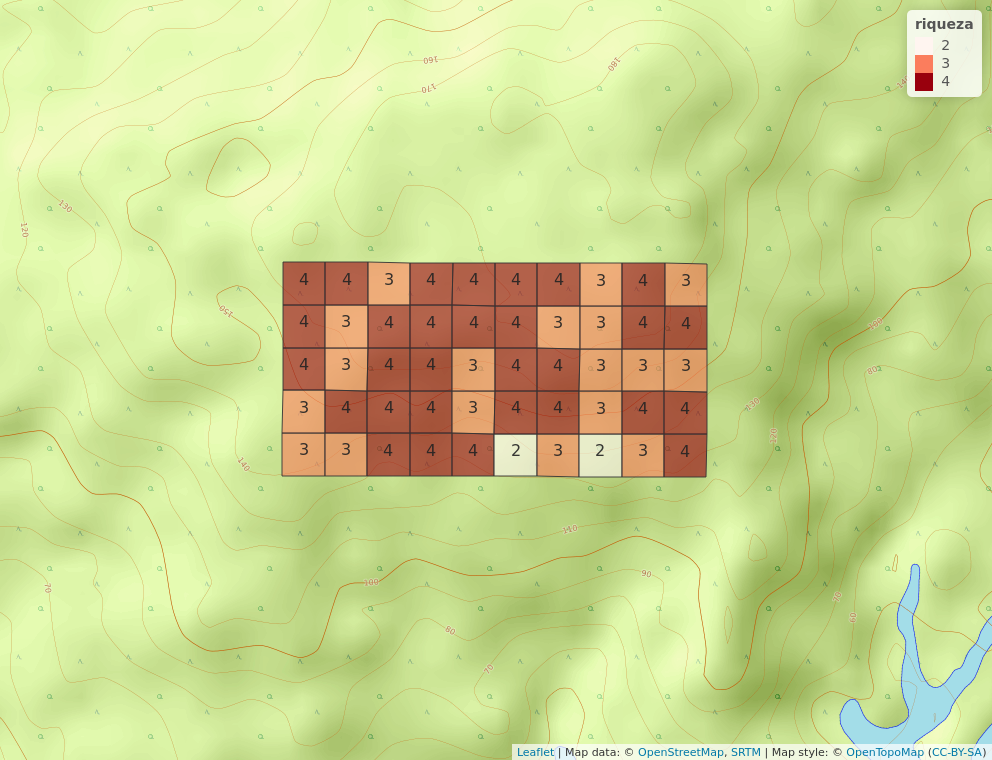
\includegraphics[width=0.50000\textwidth]{mapa_cuadros_riq_mi_familia.png}
\caption{Distribucion de la riqueza de la familia
Sapotaceae\label{fig:mapa_cuadros_riq_mi_familia}}
\end{figure}

La variables ambientales pH y pendiente media presentaron una
distribucion un tanto parecida a la disdtribución de la familia
sapotaceae. Sin embargo, la distribucion del PH esta representada mas al
oeste, mientras que la pendiente media esta distribuida en casi toda el
area, pero con una mayor concentración en la parte sur. Lo cual, se
podria decir, que la pendiente media presenta mas asocacion con la
distribución de la familia sapotaceae(ver figuras
\ref{fig:mapa_cuadros_pH} y \ref{fig:mapa_cuadros_pendiente}).

\begin{figure}
\centering
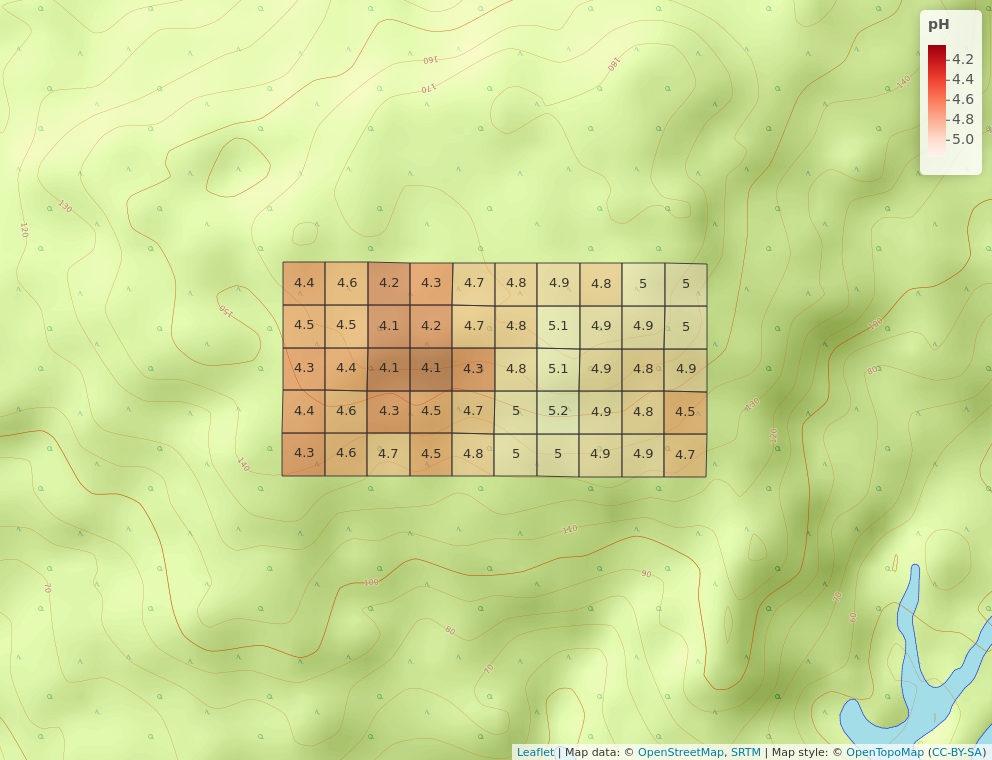
\includegraphics[width=0.50000\textwidth]{mapa_cuadros_ph.png}
\caption{Distribucion del pH\label{fig:mapa_cuadros_pH}}
\end{figure}

\begin{figure}
\centering
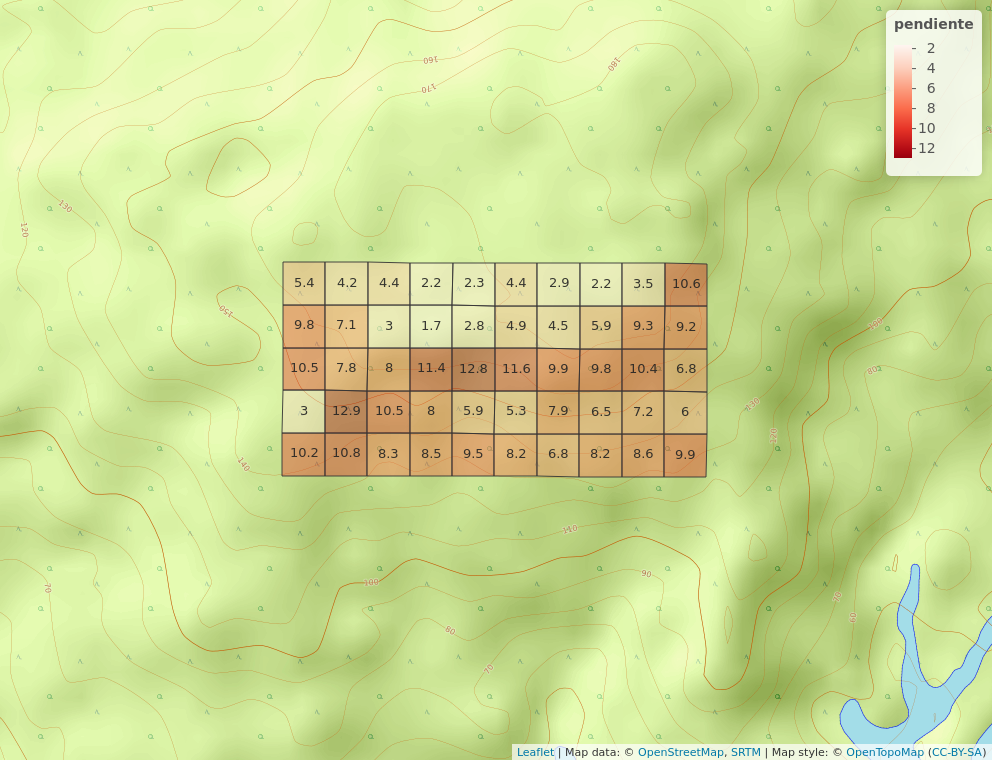
\includegraphics[width=0.50000\textwidth]{mapa_cuadros_pendiente.png}
\caption{Distribucion de las pendientes(en
grados)\label{fig:mapa_cuadros_pendiente}}
\end{figure}

la abundancia de la familia sapotaceae solo presenta correlacion con la
abundacia global, mientras que la riqueza tiene correlacion con la
presencia de cobre y nitrogeno en el suelo, lo que sugiere, que mientras
mas concentracion de cobre y nitrogeno hay, mayor será la riqueza de
especies (ver figura \ref{fig:p_cor_suelo_ar}). las variables
ambientales númericas y nominales presentaron un patrón diferente, ya
que las variables ambientales númericas tienen una distribución
heterogénea, y la distribución de las variables ambientales nominales es
mas homogena, a excepción de la variable hábita, que presenta diferentes
tipos de habitats o una distribución heterogénea(ver figuras
\ref{fig:mapas_variables_ambientales_numericas} y
\ref{fig:mapas_variables_ambientales_nominales}).

\begin{figure}
\centering
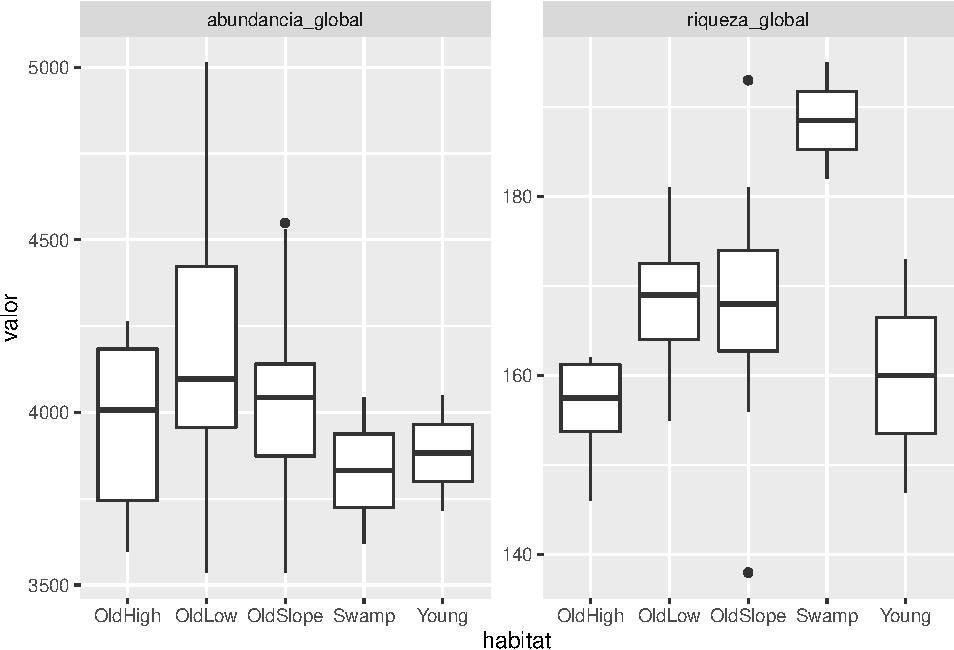
\includegraphics{manuscrito_files/figure-latex/unnamed-chunk-4-1.pdf}
\caption{\label{fig:p_cor_suelo_ar}correlacion de las variables del
suelo}
\end{figure}

\begin{figure}
\centering
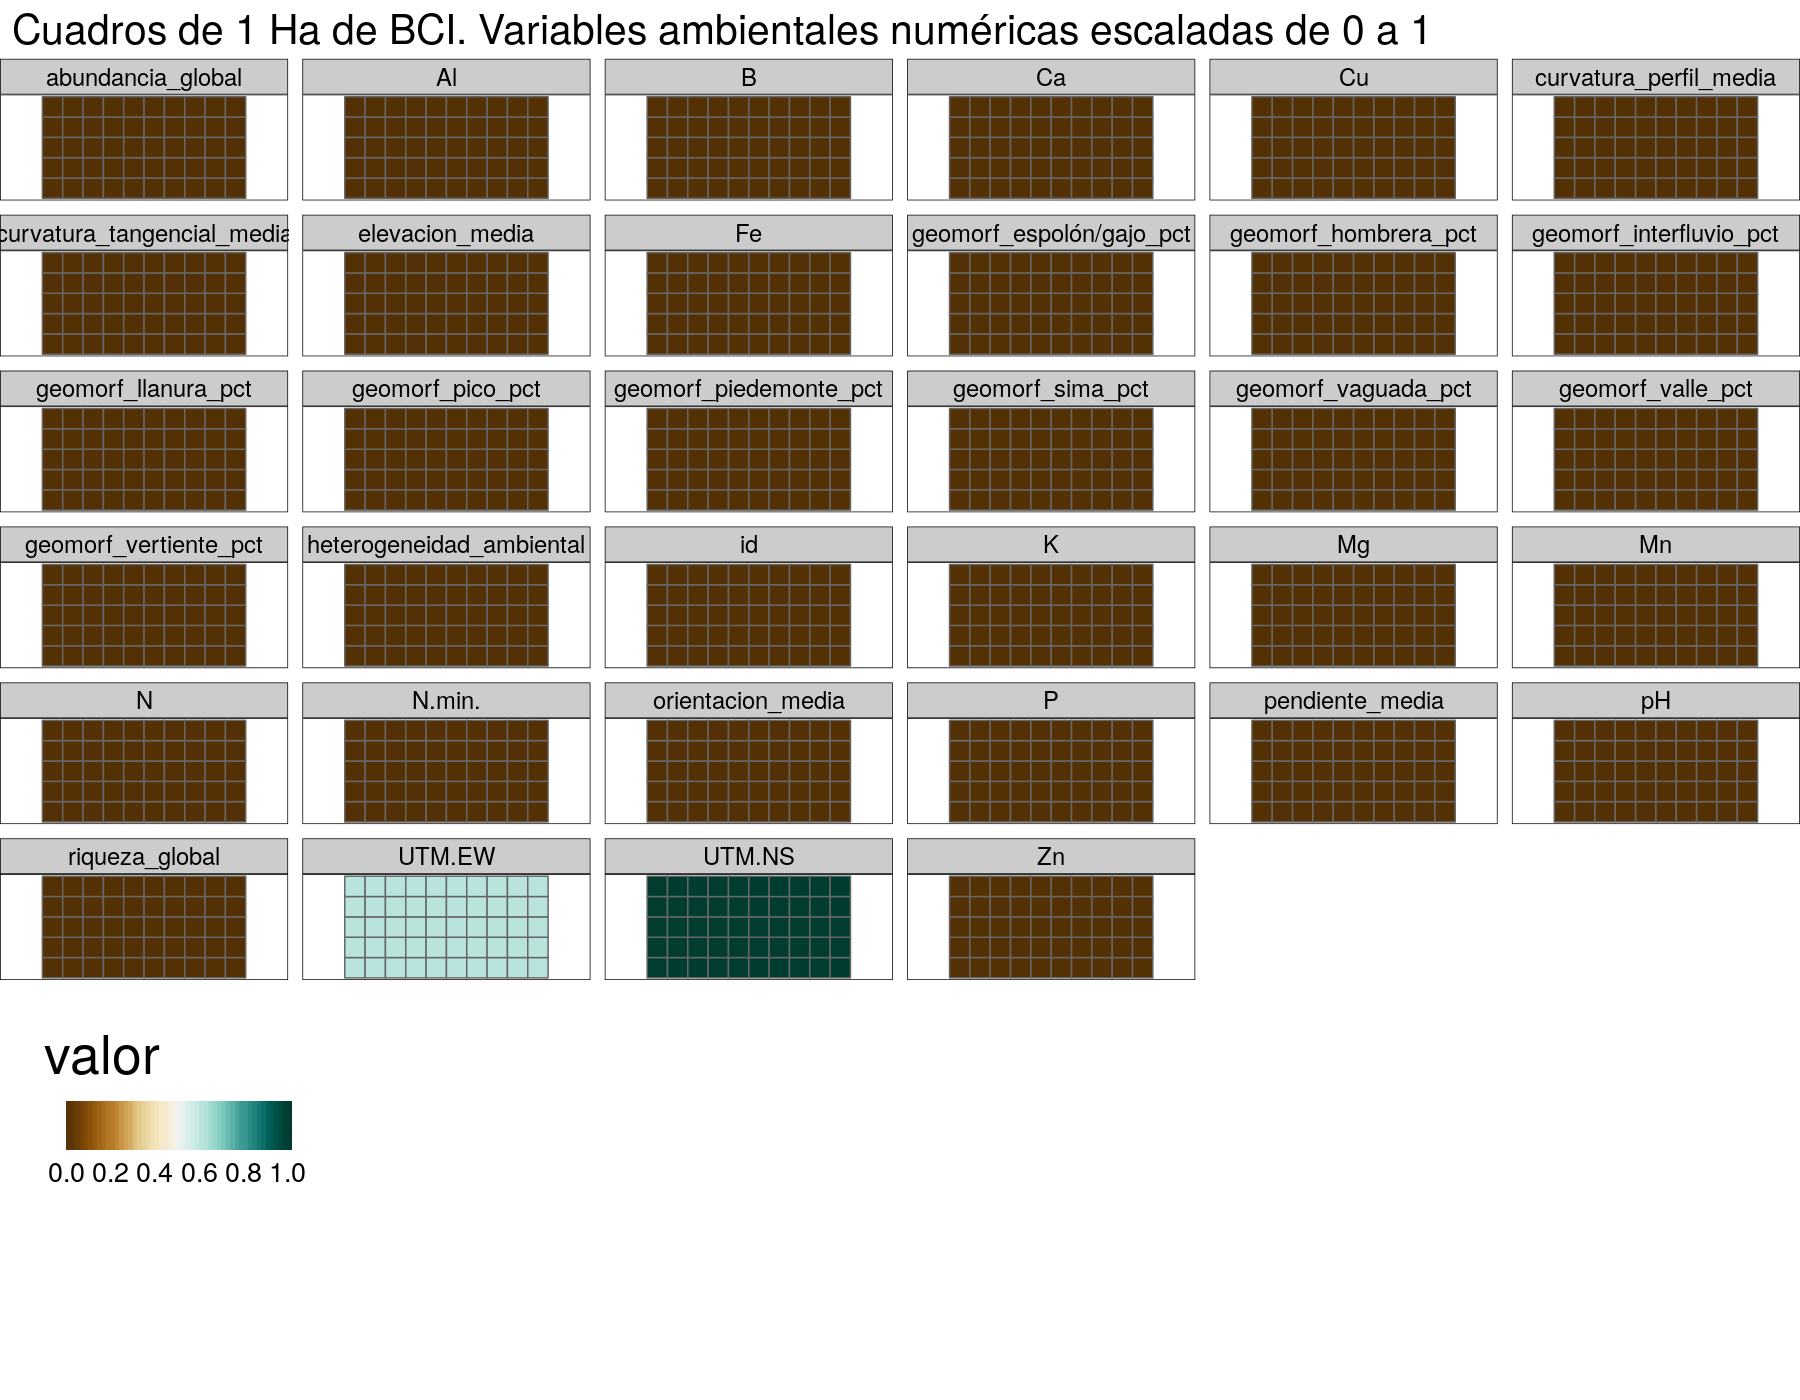
\includegraphics[width=1.00000\textwidth]{mapas_variables_ambientales_numericas_tmap.png}
\caption{variables ambientales
numericas\label{fig:mapas_variables_ambientales_numericas}}
\end{figure}

\begin{figure}
\centering
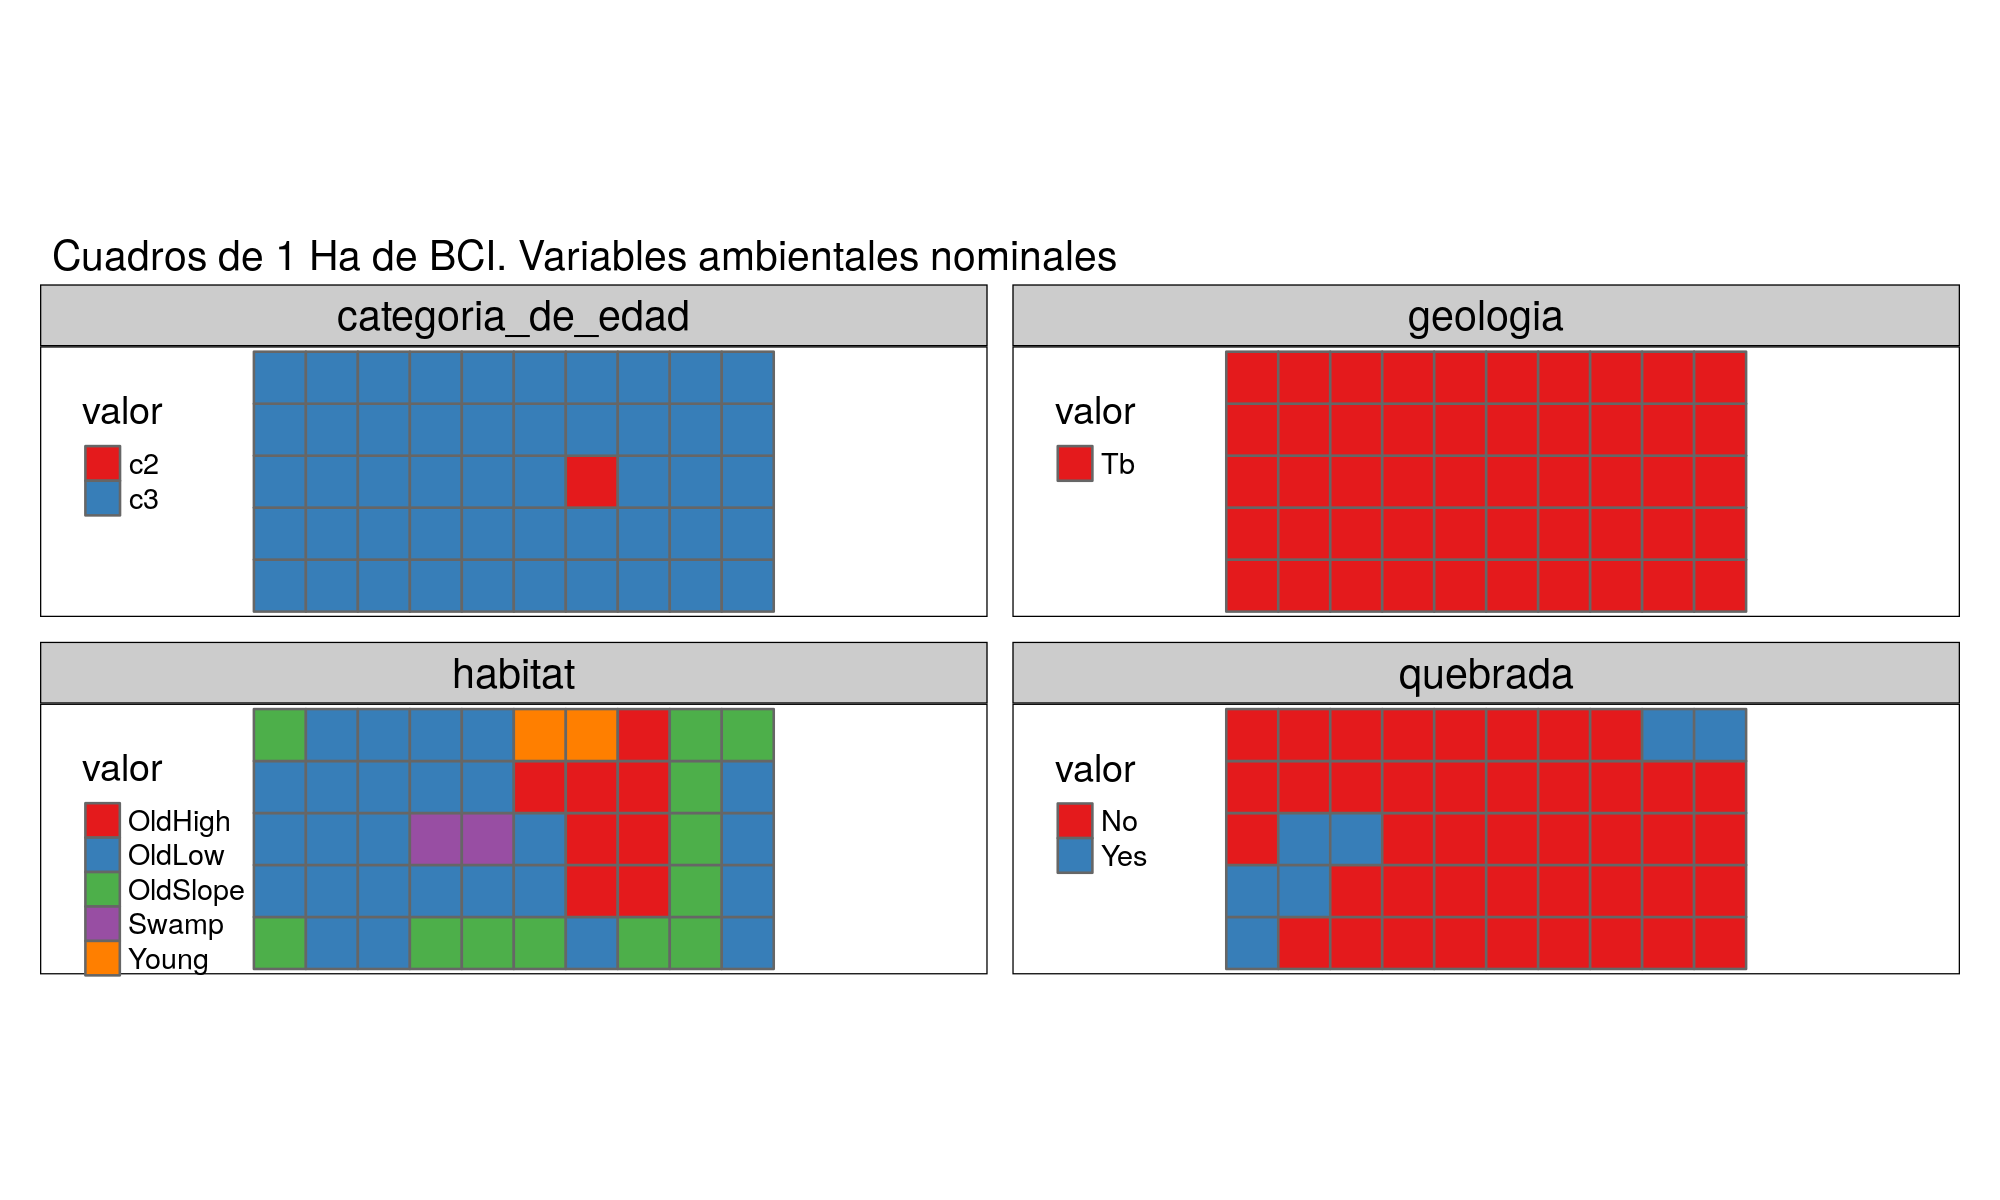
\includegraphics{mapas_variables_ambientales_nominales_tmap.png}
\caption{variables ambientales
nominales\label{fig:mapas_variables_ambientales_nominales}}
\end{figure}

El indice de similaridad de Jaccard muestra que el sitio 1 y 2 comparten
un 100\% de sus especies, por lo que ambos sitios comparten 3 especies y
no tienen especies exclusivas (ver figura
\ref{fig:similaridad_jaccard}). Las variables geomorfologicas presentan
asociación con la abundancia y riqueza, lo cual la figura
\ref{fig:matriz_correlacion_geomorf_abun_riq_spearman}, muestra que hay
mucha similaridad entre estas variables. Las pruebas de correlación
entre los grupos 1 y 2 formulados por upgma resultaron significativas
respecto a la variable fósforo. Por otro lado, el contenido de cobre y
la abundancia global promedio, es decir, la media correspondiente a
todas las plantas en BCI, son significativamente diferentes entre los
sitios de ambos grupos, para un nivel de significancia de a = 0.1(ver
figura \ref{fig:grupos_upgma}).

El grupo 1 generado por enlace upgm esta conformado por 5 cuadrante y el
grupo 2 por 46 cuadrantes (ver figura \ref{fig:mapa_upgma_k2}). El grupo
2 contiene los sitios con tendencia a presentar valores altos de zinc y
contenido de cobre. Es probable que las especies indicadoras del grupo
con un mayor contenido de cobre estén mostrando preferencia por estas
condiciones ambientales.No obstante, la mayoría de componentes del suelo
en BCI tienen valores bastante homogéneos, y más bien se presentan
pequeños gradientes entre los cuadrantes, lo cual evita que este tipo de
acercamiento sea concluyente. La especie Chrysophyllum argenteum fué la
que obtuvo un valor alto de confianza al examinar su potencial como
especies indicadoras del grupo 1. Para el caso del grupo 2, la especie
indicadora fué \emph{Pouteria reticulata}.

\begin{figure}
\centering
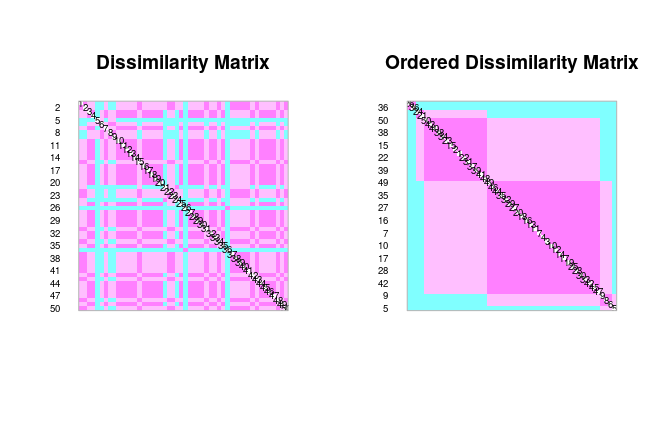
\includegraphics{medicion_asociacion_jaccard.png}
\caption{Similaridad de Jaccard(color fucsia (magenta, rosa) significa
``corta distancia=muy similares'', y cian (celeste) significa ``gran
distancia=poco similares'')\label{fig:similaridad_jaccard}}
\end{figure}

\begin{figure}
\centering
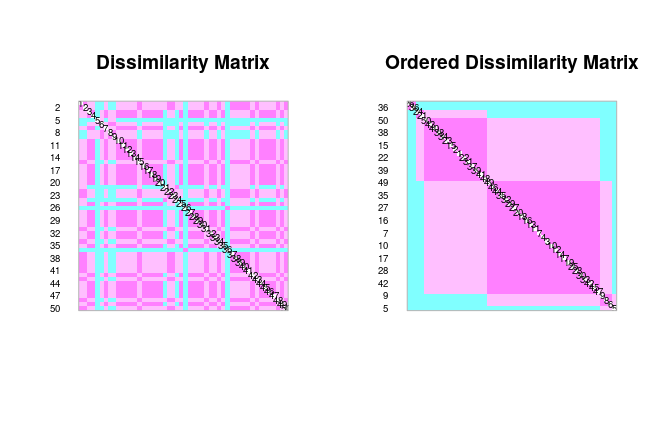
\includegraphics{medicion_asociacion_jaccard.png}
\caption{Panel de correlacion de Spearman entre los datos de la
comunidad y las variables
geomorfologicas\label{fig:matriz_correlacion_geomorf_abun_riq_spearman}}
\end{figure}

\begin{figure}
\centering
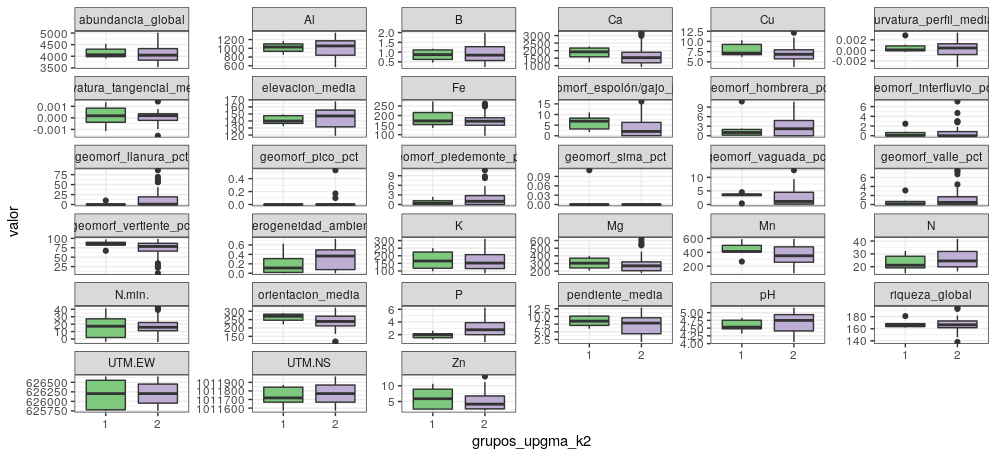
\includegraphics[width=1.00000\textwidth]{actualizacion2_grupos_upgma.png}
\caption{Diagramas de caja de las variables que tuvieron un efecto,
segun las pruebas de igualdad de medias\label{fig:grupos_upgma}}
\end{figure}

\begin{figure}
\centering
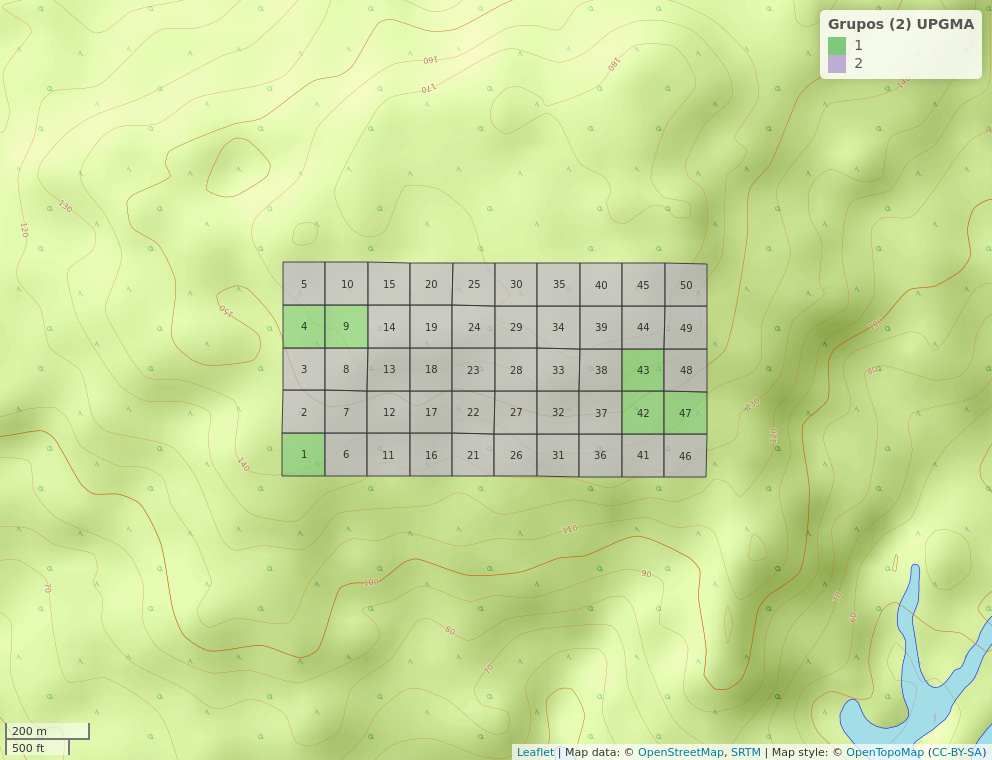
\includegraphics{mapa_upgma_k2.png}
\caption{Mapa en el que se presenta la distribucion de sitios en los
grupos formulados por enlace upgma\label{fig:mapa_upgma_k2}}
\end{figure}

La riqueza de la familia Sapotaceae aumenta en función del contenido de
hidrogeno, nitrógeno y cobre. Ademas, aunmenta con la equidad (ver
figura \ref{fig:correlacion_diversidad_equidad}). Cabe destacar, que
casi todos lo sitios de BCI tienen valores altos de equidad (ver figura
\ref{fig:grafico_niveles_equidad}). La Curva de rarefaccion de los
sitios, muestra como va aumentando la cantidad de individuos y de
especies de los cuadrantes (ver figura \ref{fig:Curva_rarefaccion}),
donde la mayor concentracion de individuos está entre los 20 a 50
individuos y la abundancia maxima es de 70 individuos. Los valores de
los indices de diversidad alfa fueron: Species Richness 0.217, Shannon
diversity 0.045 y Simpson diversity 0.038, lo cual sugiere que la
familia Sapotaceae no presenta mucha diversidad en BCI. Se estima que la
riqueza seguiria constante o no aumentaria significativamente aunque se
hiciera mayor esfuerzo de muestreo (ver
figura\ref{fig:acumulacion_especies_individuos}).

\begin{figure}
\centering
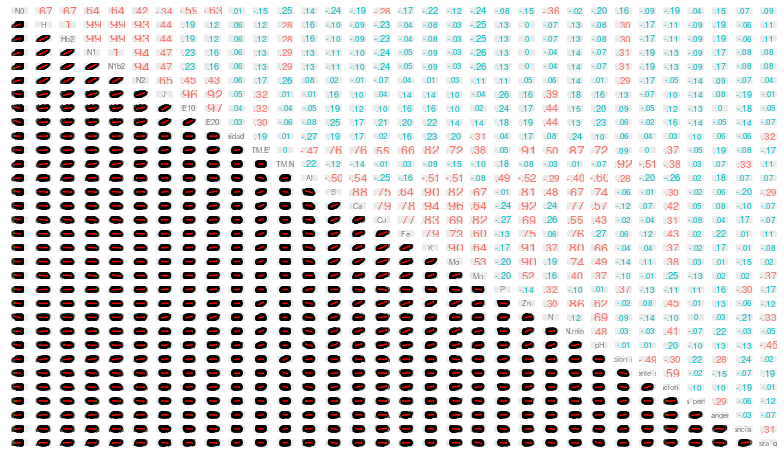
\includegraphics[width=1.00000\textwidth]{correlacion_diversidad_equidad_actualizado.png}
\caption{Correlacion entre diversidad/equidad y algunas de las variables
ambientales \label{fig:correlacion_diversidad_equidad}}
\end{figure}

\begin{figure}
\centering
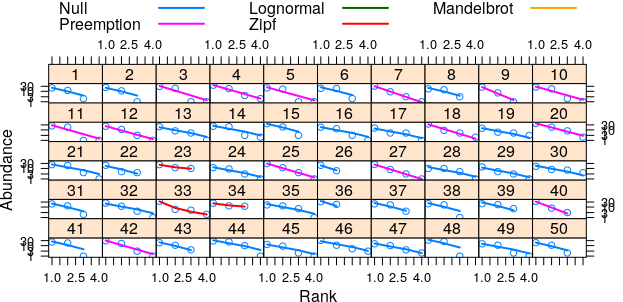
\includegraphics{grafico_niveles_equidad.png}
\caption{Grafico dque presenta los valores de equidad por sitos
\label{fig:grafico_niveles_equidad}}
\end{figure}

\begin{figure}
\centering
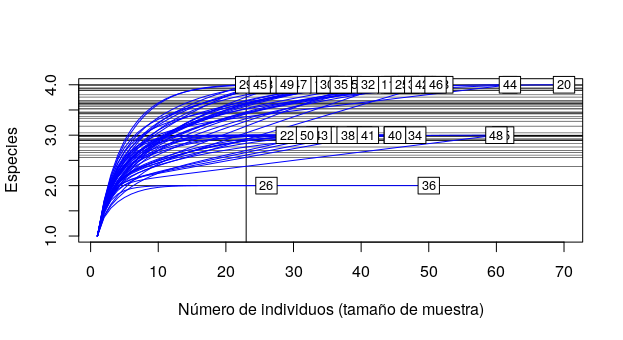
\includegraphics{Curva_rarefaccion.png}
\caption{Curva de rarefaccion de los sitios
\label{fig:Curva_rarefaccion}}
\end{figure}

\begin{figure}
\centering
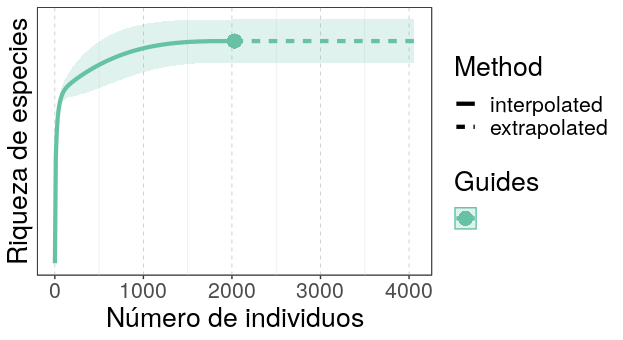
\includegraphics{acumulacion_especies_individuos.png}
\caption{Grafico de acumulacion de especies en funcion de numeros de
individuos \label{fig:acumulacion_especies_individuos}}
\end{figure}

Las especies que contribuyen de manera significativa a la diversidad
beta fueron: \emph{Chrysophyllum argenteum} (0.2504234),
\emph{Chrysophyllum cainito} (0.3147978) y \emph{Pouteria stipitata}
(0.2658814), de las cuales la que mas contribuyó a la diversidad beta
fué \emph{Chrysophyllum cainito}. No obstante, los sitios que
contribuyen a la diversidad beta son los cuadrantes 9 y 40, lo cual
presentan contribucion a la diversidad beta por la incidencia de algunas
variables ambientales (ver figura
\ref{fig:mapas_variables_ambientales_numericas} y
\ref{fig:mapas_variables_ambientales_nominales}).

El grafico \ref{fig:env_suelo_pca} incluye el comportamiento de los
componentes principales de la varianza en las variables suelo y
geomorfologia en BCI, predecido por el modelo de barra quebrada,
representado por la línea roja formando la curva (La escala denominada
``Inertia'' representa la suma de los cuadrados de toda la varianza). En
el diagrama rotulado como escalamiento 1 de la figura
\ref{fig:Biplot_PCA_escalamiento}, se observan tres grupos de cuadrantes
diferenciados entre sí. Un grupo de sitios con un alto grado de acidez y
contenido en aluminio, otro grupo caracterizado por la presencia de
elementos metálicos, y un tercero, con una cantidad de fósforo,
nitrógeno y valor de pH mayor. Las variables nitrógeno, fósforo y pH
aportan la mayor parte de la varianza explicada. La relación entre las
variables se encuentra debidamente representada en el recuadro del
escalamiento 2, por medio de los ángulos que forman sus vectores (ver
figura \ref{fig:Biplot_PCA_escalamiento}).

\begin{figure}
\centering
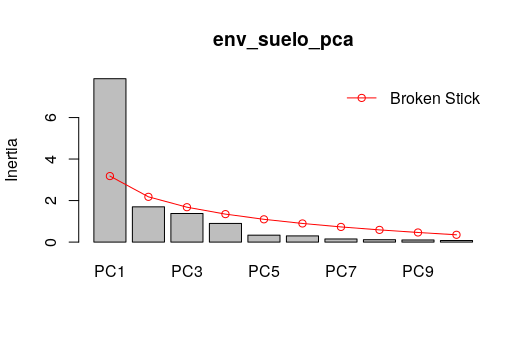
\includegraphics{env_suelo_pca.png}
\caption{grafico de los componentes principales de la varianza en las
variables suelo y geomorfologia en BCI \label{fig:env_suelo_pca}}
\end{figure}

\begin{figure}
\centering
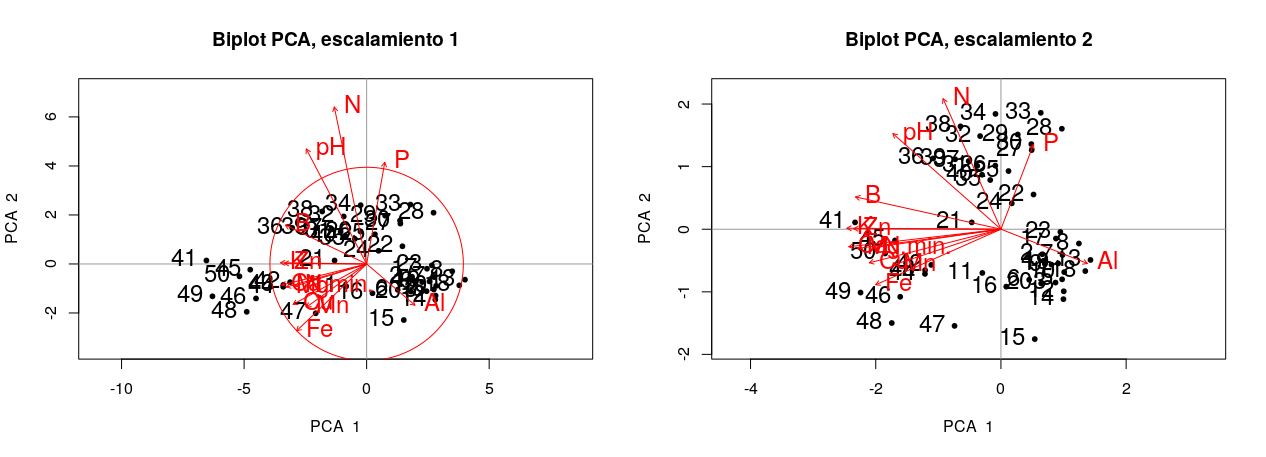
\includegraphics[width=1.00000\textwidth]{Biplot_PCA_escalamiento_actualizado.png}
\caption{Biplots generados en el PCA de las viariables de suelo
\label{fig:Biplot_PCA_escalamiento}}
\end{figure}

Los resultados del PCA de los datos de la matriz de comunidad se
encuentran resumidos en los diagramas de la figura
\ref{fig:PCA_comunidad}. El escalamiento 1, muestra muchos de los
cuadrantes dispuestos alrededor del origen formado por los ejes, lo que
indica una contribución a la varianza relativamente equitativa por parte
de las especies.

\begin{figure}
\centering
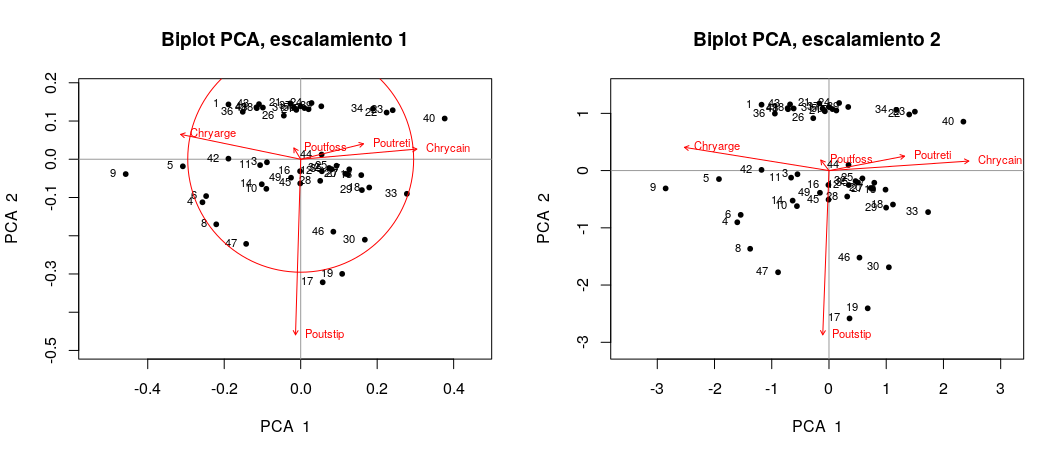
\includegraphics[width=1.00000\textwidth]{PCA_comunidad_actualizado.png}
\caption{Biplots generados en el PCA de las viariables de suelo
\label{fig:PCA_comunidad}}
\end{figure}

El escalamiento 2 de la figura \ref{fig:Analisis_de_correspondencia} en
el análisis de correspondencia mostró que las especies Pouteria
reticulata, Chrysophyllum argenteum y Chrysophyllum cainito se
encuentran asociadas. Estas especies, además, tienen los valores mas
altos de abundancia dentro de la comunidad (1084, 711 y 171 individuos,
respectivamente). Las especies restantes tienen una abundancia reducida,
y en consecuencia, aparecen cercanas a los pocos cuadrantes en los que
se encuentran representadas. La disparidad en la incidencia de las
especies se refleja en su disposición en el diagrama. Sin embargo, estos
resultados no coinciden del todo con los arrojados por el PCA de la
matriz de distancias.

\begin{figure}
\centering
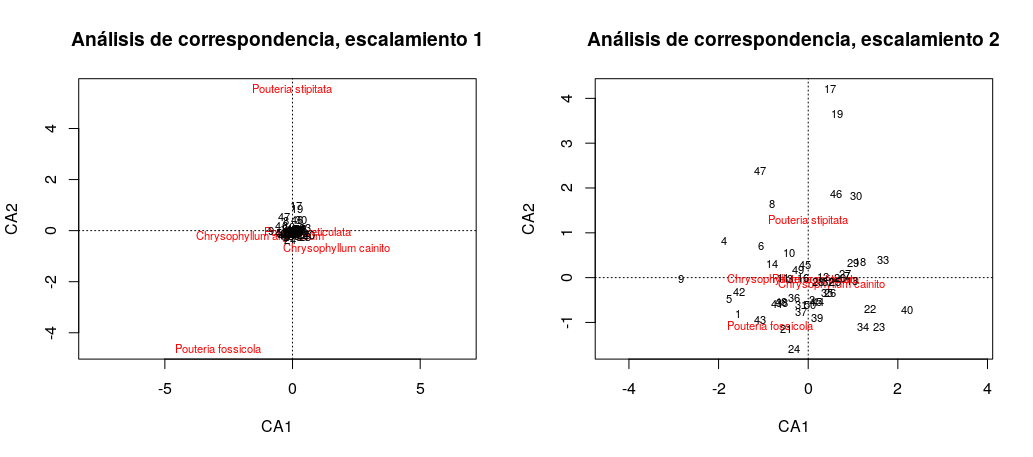
\includegraphics[width=1.00000\textwidth]{analisis_de_correspondencia_actualizado.png}
\caption{Biplot del analisis de correspondencia de los datos de
abundancia de las especies de Sapotaceae
\label{fig:Analisis_de_correspondencia}}
\end{figure}

Los primero ordenes de \emph{Chrysophyllum argenteum} y
\emph{Chrysophyllum cainito} presentan valores de autocorrelacion alta o
positiva, mientras que los ordenes de las demas especies presentan
mayormente valores de autocorrelacion negativa, teniendo en cuenta que
el orden 5 de todas las especies presenta autocorrelacion negativa, lo
que sugiere que orden 5 de las especies está autocorrelacionado
espacialmente negativo (Ver figura \ref{fig:Abundancia_matriz}.

\begin{figure}
\centering
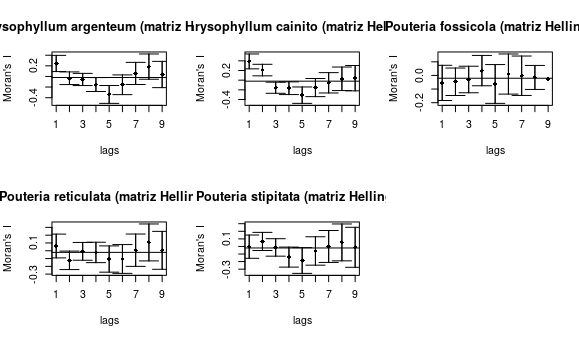
\includegraphics[width=1.00000\textwidth]{Abundancia_matriz.png}
\caption{Autocorrelación espacial de las especies
\label{fig:Abundancia_matriz}}
\end{figure}

\section{Discusión}\label{discusiuxf3n}

\section{Agradecimientos}\label{agradecimientos}

\section{Información de soporte}\label{informaciuxf3n-de-soporte}

\ldots

\section{\texorpdfstring{\emph{Script}
reproducible}{Script reproducible}}\label{script-reproducible}

\section*{Referencias}\label{referencias}
\addcontentsline{toc}{section}{Referencias}

\hypertarget{refs}{}
\hypertarget{ref-jose_ramon_martinez_batlle_2020_4402362}{}
Batlle, J. R. M. (2020). biogeografia-master/scripts-de-analisis-BCI:
Long coding sessions (Version v0.0.0.9000).
\url{https://doi.org/10.5281/zenodo.4402362}

\hypertarget{ref-brocard2011numerical}{}
Brocard, D., Gillet, F., \& Legendre, P. (2018). Numerical ecology with
r. \emph{Springer Nature}, \emph{Second Edition}, 52--66. Retrieved from
\url{https://doi.org/10.1007/978-3-319-71404-2}

\hypertarget{ref-carmona2013diversidad}{}
Carmona-Galindo, V. D., \& Carmona, T. V. (2013). La diversidad de los
análisis de diversidad la diversidad de los analisis de diversidad
{[}the diversity of diversity analyses{]}. \emph{Bioma}.

\hypertarget{ref-caceres2009associations}{}
Cáceres, M. D., \& Legendre, P. (2009). Associations between species and
groups of sites: Indices and statistical inference. \emph{Ecology},
\emph{90}(12), 3566--3574.

\hypertarget{ref-condit2012thirty}{}
Condit, R. A. y H., Richard y Chisholm. (2012). Treinta años de censo
forestal en barro colorado y la importancia de la inmigración para
mantener la diversidad. \emph{PloS One}, \emph{7}(11), e49826.

\hypertarget{ref-condit2017demographic}{}
Condit, R. y L., Richard y P ~'e rez. (2017). Tendencias demográficas y
clima durante 35 años en la parcela de 50 ha de barro colorado.
\emph{Forest Ecosystems}, \emph{4}(1), 1--13.

\hypertarget{ref-dufrene1997species}{}
Conjuntos de especies y especies indicadoras: La necesidad de un enfoque
asimétrico flexible. (1997). \emph{Monografías Ecológicas},
\emph{67}(3), 345--366.

\hypertarget{ref-croat1978flora}{}
croata, T. B. (1978). \emph{Flora de la isla barro colorado}. Stanford
University Press.

\hypertarget{ref-indicspecies}{}
De Caceres, M., \& Legendre, P. (2009). Associations between species and
groups of sites: Indices and statistical inference. In \emph{Ecology}.
Retrieved from \url{http://sites.google.com/site/miqueldecaceres/}

\hypertarget{ref-fisher1943relation}{}
Fisher, R. A., Corbet, A. S., \& Williams, C. B. (1943). The relation
between the number of species and the number of individuals in a random
sample of an animal population. \emph{The Journal of Animal Ecology},
42--58.

\hypertarget{ref-leigh1990barro}{}
Isla barro colorado y biología tropical. (1990). \emph{Cuatro Bosques
Neotropicales}, 28--47.

\hypertarget{ref-diversityanalysis}{}
Kindt, R., \& Coe, R. (2005). \emph{Tree diversity analysis. a manual
and software for common statistical methods for ecological and
biodiversity studies}. Retrieved from
\url{http://www.worldagroforestry.org/output/tree-diversity-analysis}

\hypertarget{ref-legendre2001ecologically}{}
Legendre, P., \& Gallagher, E. D. (2001). Ecologically meaningful
transformations for ordination of species data. \emph{Oecologia},
\emph{129}(2), 271--280.

\hypertarget{ref-martinez2020importancia}{}
Martínez-Sovero, G., Iglesias-Osores, S., \& Villena-Velásquez, J. J.
(2020). Importancia de la familia sapotaceae en madre de dios, perú.
\emph{Manglar}, \emph{17}(4), 287.

\hypertarget{ref-martinez2021diversidad}{}
Martínez-Sovero, G., Iglesias-Osores, S., Muñoz-Chavarry, P.,
Seminario-Cunya, A., Alva-Mendoza, D., \& Villena-Velásquez, J. (2021).
Diversidad y estructura de sapotaceae en bosques amazónicos de madre de
dios, perú. \emph{Ciencia Amazónica (Iquitos)}, \emph{9}(1), 59--72.

\hypertarget{ref-vegan}{}
Oksanen, J., Blanchet, F. G., Friendly, M., Kindt, R., Legendre, P.,
McGlinn, D., \ldots{} Wagner, H. (2019). \emph{Vegan: Community ecology
package}. Retrieved from \url{https://CRAN.R-project.org/package=vegan}

\hypertarget{ref-perez2005metodologia}{}
Pérez, R., Aguilar, S., Condit, R., Foster, R., Hubbell, S., \& Lao, S.
(2005). Metodologia empleada en los censos de la parcela de 50 hectareas
de la isla de barro colorado, panamá. \emph{Centro de Ciencias
Forestales Del Tropico (CTFS) Y Instituto Smithsonian de Investigaciones
Tropicales (STRI)}, 1--24.

\hypertarget{ref-Restudio}{}
R Core Team. (2020). \emph{R: A language and environment for statistical
computing}. Retrieved from \url{https://www.R-project.org/}

\hypertarget{ref-rodriguez2020scolytinae}{}
Rodríguez-Flores, W., \& Barrios, H. (2020). Scolytinae y platypodinae
(coleoptera: Curculionidae) de la isla barro colorado, panamá.
\emph{Scientia}, \emph{30}(1), 15--52.

\hypertarget{ref-shannon1948mathematical}{}
Shannon, C. E. (1948). Una teoría matemática de la comunicación.
\emph{El Diario Técnico Del Sistema Bell}, \emph{27}(3), 379--423.

\hypertarget{ref-simpson1949measurement}{}
Simpson, E. H. (1949). Measurement of diversity. \emph{Nature},
\emph{163}(4148), 688--688.

\hypertarget{ref-smedmark2007boreotropical}{}
Smedmark, A. A., Jenny EE y Anderberg. (2007). La migración
boreotropical explica la hibridación entre linajes geográficamente
distantes en el clado pantropical sideroxyleae (sapotaceae).
\emph{American Journal of Botany}, \emph{94}(9), 1491--1505.

\hypertarget{ref-whittaker1960vegetation}{}
Whittaker, R. H. (1960). Vegetation of the siskiyou mountains, oregon
and california. \emph{Ecological Monographs}, \emph{30}(3), 279--338.

\hypertarget{ref-tidyverse}{}
Wickham, H. (2017). \emph{Tidyverse: Easily install and load the
'tidyverse'}. Retrieved from
\url{https://CRAN.R-project.org/package=tidyverse}

\hypertarget{ref-windsorestructura}{}
Windsor, D., FOSTER, R., BROKAW, N., Leigh, E., Rand, A., \& others.
(n.d.). \emph{Estructura e historia de la vegetación de la isla barro
coloradoecología de un bosque tropical: Ciclos estacionales y cambios a
largo plazo}.




\newpage
\singlespacing 
\end{document}
